\documentclass{article}
\title{Project 3 \\ FYS-STK3155/4155}
\author{Magnus Bergkvam}
\usepackage{url}
\usepackage{amsmath}
\usepackage{graphicx}
\usepackage{subfig}
\usepackage{bm}
\usepackage{listings}

\graphicspath{{../figures/}}


\begin{document}
\maketitle
\bibliographystyle{unsrt}

\section{Abstract}
Machine learning classifiers have many important uses, from spam classification
of emails, to image classification in the medical sector and much more. They
also have found use for quite important and high-risk tasks like credit-card
fraud detection \cite{creditcardfraud}, where a good classifier is important
for as many credit-card frauds to be stopped as possible, while at the same
time legitimate payments going through.

In this project we explored how different models performed on a data-rich
credit-card fraud dataset \cite{kaggleccdata}. For this we looked at three
different types of models, one being a simple logistic regression, another one
being neural networks and finally we looked at gradient-boosted decision trees.
Unlike the previous projects we have just used established machine-learning
libraries namely sklearn, tensorflow and xgboost for the models and done
parameter tuning on each of the models. What we found was that the logistic
regression did manage to classify most predictions at $96\%$ overall accuracy
on the test-data, however it still performed considerably worse than the other
two models. For the neural network we ended up with a model with two hidden
layers, each with $100$ nodes, using the RMSProp optimizer, with some $l_2$
regularization and relu activation functions. The neural network did give us
quite good classification with it being able to correctly classify all the
fraud cases, and only giving $62$ false positives out of more than $35 000$
observations. The best performance though was the gradient boosted decision
tree, also correctly classifying all the fraud cases and only giving $21$ false
positives.

Overall this project has shown that for credit card fraud detection, gradient
boosting especially, but also neural networks, are both very good classifiers
for this task. This effect likely translates into other data-rich binary
classification cases as well.

\section{Introduction}
Credit card fraud detection is one of many application where machine learning
binary-classification models are widely used. Furthermore it is a case where
having a good classifier is essential for the credit-card system to work in the
first place. It is important that the vast majority of legitimate purchases are
detected as legitimate as reliability of use of credit cards is quite important
if you want people to use your credit cards. For example, when going to the
store and buying something you shouldn't have to worry at all about the card being
declined. At the same time it is perhaps even more important that the actual
frauds are detected as such, as the credit-card company can then take action to
block the payments and maybe even the card. This is both important for the user
of the credit card and the issuer, as it can be a huge hurdle for the owner if
fraud payments are not detected and go through normally, which is both
uncomfortable and time-consuming. Additionally for the issuer, the more fraud
payments they let go through, the more payments they potentially have to cover
themselves.

What is clear is then that a very good classifier is needed in order to limit
these situations discussed. We will here try to explore some different models
for classifying fraud and see how good they perform. The dataset we will be
using contains more than $550 000$ transactions, each with $28$ anonymized
features plus the amount spent, and a binary response representing fraud or not
fraud. We will focus mainly on three types of models. The simplest one being
logistic regression, then we will go back to neural networks as we found that
they performed very well in project 2 \cite{githubrepoproject2} and finally
we'll look at a decision tree, more specifically a gradient boosting tree.

A motivation behind using logistic regression is that as we have already seen,
they often can perform rather well on less complex problems, due to their low
complexity (low variance). On problems like these this usually can't compete
with the other two models, but we will see how big of a gap we'll get between
them, and this can also serve as some sort of benchmark for the other two
models. Neural networks is a good choice for a lot of problems, with them being
very general and often perform well when we have a lot of data. Boosting trees
we have chosen to bring in here because they very often are a go-to for
classification purposes, with them being the winner of many classification
competitions. Additionally they are more intuitive than the neural network
approach, and less computationally expensive.

We'll first in the method introduce some of the models we'll use, and go
through the data a bit closer, before we look at how the three different models
perform, and from there on we will try to conclude which of the three models
performs the best for this data and try to put into perspective just how good
they perform, and if it is good enough.

\section{Methods}
\subsection{The credit card fraud data}
At the heart of all our experimentation is the credit-card fraud detection
data from 2023 \cite{kaggleccdata}. This is a dataset where each observation
corresponds to one transaction. Luckily for our predictions as well, this is
quite rich on data with there being $568630$ total observations/transactions.
Furthermore this data is equally split among the two classes, with there being
$284315$ non-fraudulent and fraudulent transactions each. This is probably
going to be a good thing for our models, as the models has then as much
information of what constitutes a fraudulent transaction, as a non-fraudulent
transaction.

The data is collected using transactions from European credit card holders in
the year $2023$ \cite{kaggleccdata}. The fact that we only have data collected
from Europeans does perhaps limit the performances of our models on
non-european card holders. If for example in another part of the world a
legitimate credit-card transaction typically looks different, or likewise with
fraud, our models are not guaranteed to be as good classifiers as the ones we
will get from this dataset, so this is something we will need to keep in mind.
Each transaction contains a unique identifier (labeled id), $28$ anonymized
features (labeled $\text{V}1$ to $\text{V}28$), the transaction amount (labeled
as Amount) and a categorical variable indicating whether we have a fraudulent
transaction (labeled as Class). For the Class we have that $1$ constitutes
fraud while $0$ constitutes a legitimate transaction. We will obviously not use
id id for training here, as this should not impact whether a transaction is
fraudulent, but we will use all the other variables in our models, with Class
as the binary response. Another thing which makes this data quite convenient is
that all of the features are numerical, with there being no NA/NULL values as
all, which makes the required preprocessing here very small (the only
preprocessing I'll do is scaling the rows with StandardScaler).
\\

To see some dependencies of the response for each explanatory variable we can
create a box-plot for each feature. Figure \ref{databoxplot} shows exactly
this. As we can see there are quite a few of the anonymized features especially
which looks to be distributed slightly differently for the fraudulent
transactions than the legitimate ones. This difference in distribution of some
of the features looks promising our classification.


\begin{figure}
	\centering
	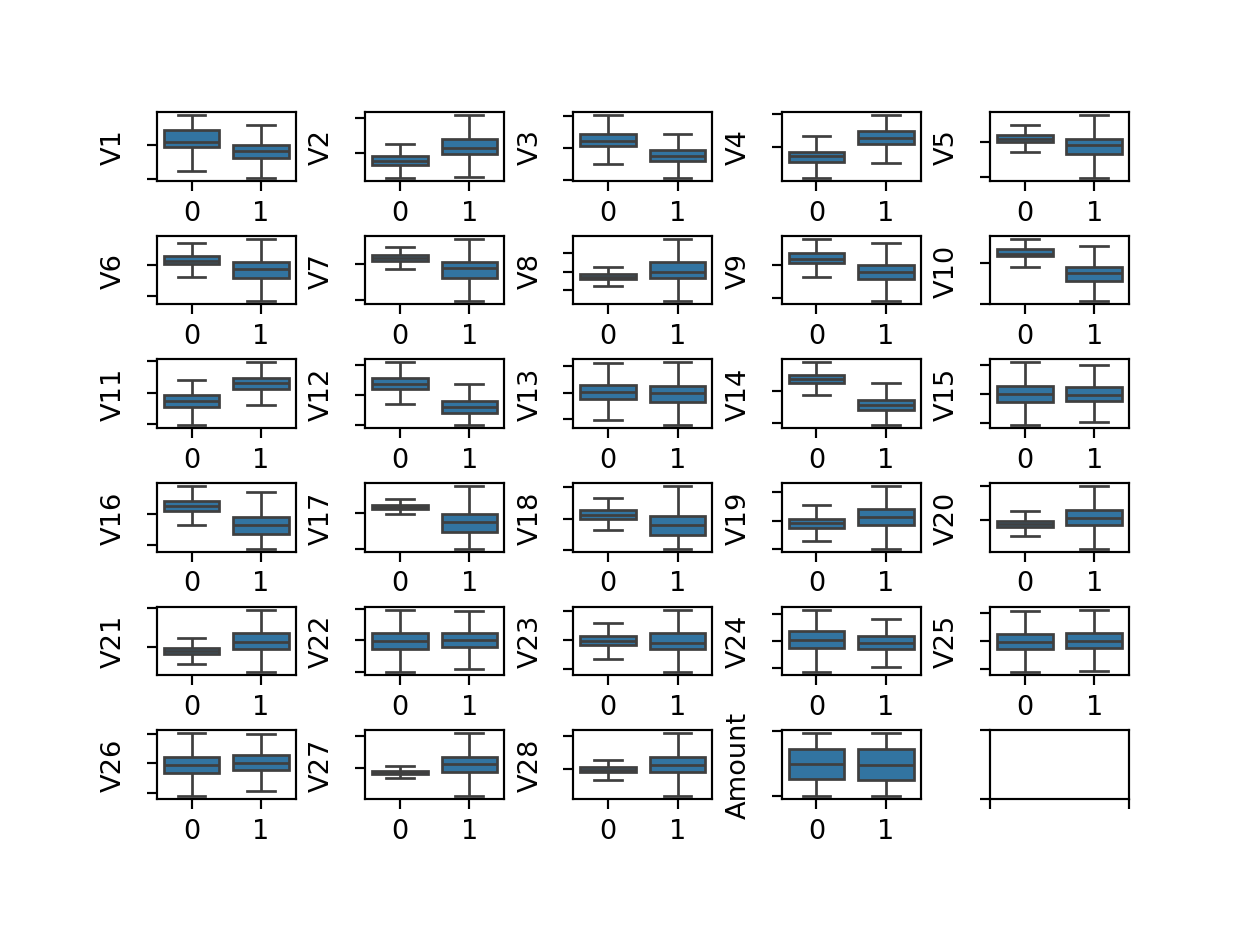
\includegraphics[scale=0.8]{data_features_boxplot}
	\caption{Shows a boxplot with each feature along the y-axis and the
		binary response on the x-axis. This plot was generated from a random
		sample of $10 000$ observations of the data. We see that for the anonymized
		features (bar 13 15 22 23 24 25 26) there seems to be a clear difference in
		distributions for the feature-values for the non-fraudulent and fraudulent
		transactions.}
	\label{databoxplot}
\end{figure}

\subsection{Neural Networks}
For the neural networks in this project we will use a basic multi-layer
perceptron, this time using tensorflow. I will assume knowledge of the basic
setup of training, and. For more details on the neural networks feel free to
check out the report of project 2 \cite{githubrepoproject2}. We will spend some
time tweaking the based on the performance based on what gives us good
performance on the validation set. Luckily for us we have a lot of data, with
the two classes being quite evenly distributed, so using this approach over
something like corss-validation should be unproblematic.

The main things we will be tweaking is the regularization parameter (we will
limit ourselves to use $l_2$ regularization), the optimization method (with the
corresponding learning-rate), the activation functions and the network size.
The output function will be fixed to be the sigmoid function in this case as we
are dealing with binary classification, while the cost-function will be binary
cross-entropy, both just as in project 2.

The optimization methods we will try in this case is just as in project 2, i.e.
AdaGrad, Adam, RMSProp and SGD. We have dropped trying out normal gradient
descent, because of it's uncompetitive performance in project 2, as well as the
fact that our dataset now will be huge, meaning that the amount of epochs we
are willing to give in the learning-process is severely limited, meaning it
should have even worse prerequisites in this case. All these are built directly
into tensorflow so the amount we need to implement here is quite limited.

For the activation-functions we will try out the relu and sigmoid (which we
already have explored in project 2), as well as some other activation functions
built into tensorflow. Notably these are swish, tanh and elu. We will now go a
little bit into these:
\subsubsection{tanh}
The tanh is given by:
$$\text{tanh}(x) = \frac{\exp(x) - \exp(-x)}{\exp(x) + \exp(-x)}$$ \cite{wikihyperbolicfunctions}
This looks much like the sigmoid function, in that is has the same s-shape, but
is different in the sense that the sigmoid limits us between $0$ and $1$, while
the tanh limits us between $-1$ and $1$. This can in some situations be
preferable.

\subsubsection{swish}
The swish is given by:
$$\text{swish}(x) = x \cdot \text{sigmoid}(x).$$ \cite{tensorflowdocswish}
Using our knowledge about the sigmoid-function we see that as $x$ grows, the
sigmoid will approach $1$ quite quickly. This means that for high values of
$x$, the function will behave much like the relu. For negative values of $x$ we
have that the sigmoid becomes very close to $0$, much quicker than the linear
function $x$ grows towards $-\infty$, so the product will be very close to $0$,
again much like the relu. However for small absolute values we will get a
shrinking in absolute value of the activations. This function often works
better than the ReLU on deep models on challenging datasets
\cite{ramachandran2017searching}, so we will explore if this is one of those
cases.

\subsubsection{ELU}
The exponential linear unit is given by:
$$\text{elu}(x) = \begin{cases} x \qquad \qquad & \text{if}\ \ x > 0 \\ \alpha \cdot (\exp(x) - 1) & \text{if}\ \ x < 0 \end{cases}.$$ \cite{tensorflowdocelu}
We will here just use $\alpha = 1$ (which is the default), but of course it is
easy to test others as well. The ELU can lead to faster learning and better
performance on neural nets with more than $5$ layers in particular
\cite{clevert2016fast}, which is less than what we mainly will be using here,
but we will try it anyway.

\subsection{Boosting trees}
This is a method we haven't been through earlier, so we'll go a little bit more
into this here. At the core of a boosting-tree is a normal classification-tree.
Often gradient boosted trees are very good for classification purposes.

\section{Results}

\section{Analysis}

\section{Conclusion}

\section{Appendix}

\subsection{Project code (github)}
All the python programs described in the report and with the full source code can be
found at:
\url{https://github.com/magnouvean/ml-physics-projects/tree/main/project3/python}

\bibliography{./sources.bib}

\end{document}
